% See http://tex.stackexchange.com/questions/168169/options-for-supplementary-materials-in-preprint-version-revtex-arxiv

\section*{Additional Files}

\setcounter{equation}{0}
\setcounter{figure}{0}
\setcounter{table}{0}
\makeatletter
\renewcommand{\theequation}{S\arabic{equation}}
\renewcommand{\thefigure}{S\arabic{figure}}

\begin{center}
    \begin{tabular}{ | l | l | l | p{5cm} |}
    \hline
    \textbf{Data File} & \textbf{Format} & \textbf{Title} & \textbf{Description} \\ \hline
    \texttt{Additional File 1.csv} & CSV & Samples & Sample identifiers, basic clinical information, specimen purities, mutation and neoantigen burden, contributions of major mutational signatures to mutations and neoantigens, and chemotherapy treatments \\ \hline

    \texttt{Additional File 2.csv.zip} & CSV zip & Mutations & Mutations, read counts, predicted effects, and resulting neoantigens \\ \hline
    
    \texttt{Additional File 3.csv} & CSV & HLA types & HLA types for each donor \\ \hline
    
    \texttt{Additional File 4.csv} & CSV & Mutational signatures & COSMIC curated signatures and the extracted chemotherapy signatures \\ \hline

    \texttt{Additional File 5.csv} & CSV & Signature deconvolutions & Results of mutational signature deconvolution for all samples, including separate analyses of all mutations and mutations unique to the treated paired samples  \\ \hline
    
    \texttt{Additional File 6.csv} & CSV & Shared neoantigens & Neoantigens predicted for multiple patients  \\ \hline
    \end{tabular}
\end{center}


\section*{Supplemental Figures}

\begin{figure}
\centering
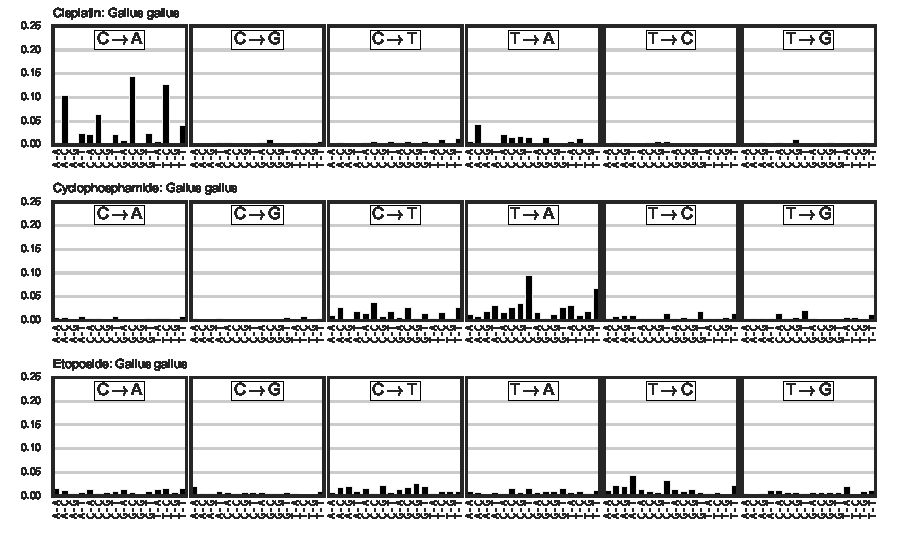
\includegraphics[scale=1.0]{figures/extracted_signatures_chicken.pdf}
\caption{Mutational signatures extracted from Szikriszt et al.~\cite{Szikriszt_2016}}
\label{fig:supp_extracted_signatures_chicken}
\end{figure}

\begin{figure}
\centering
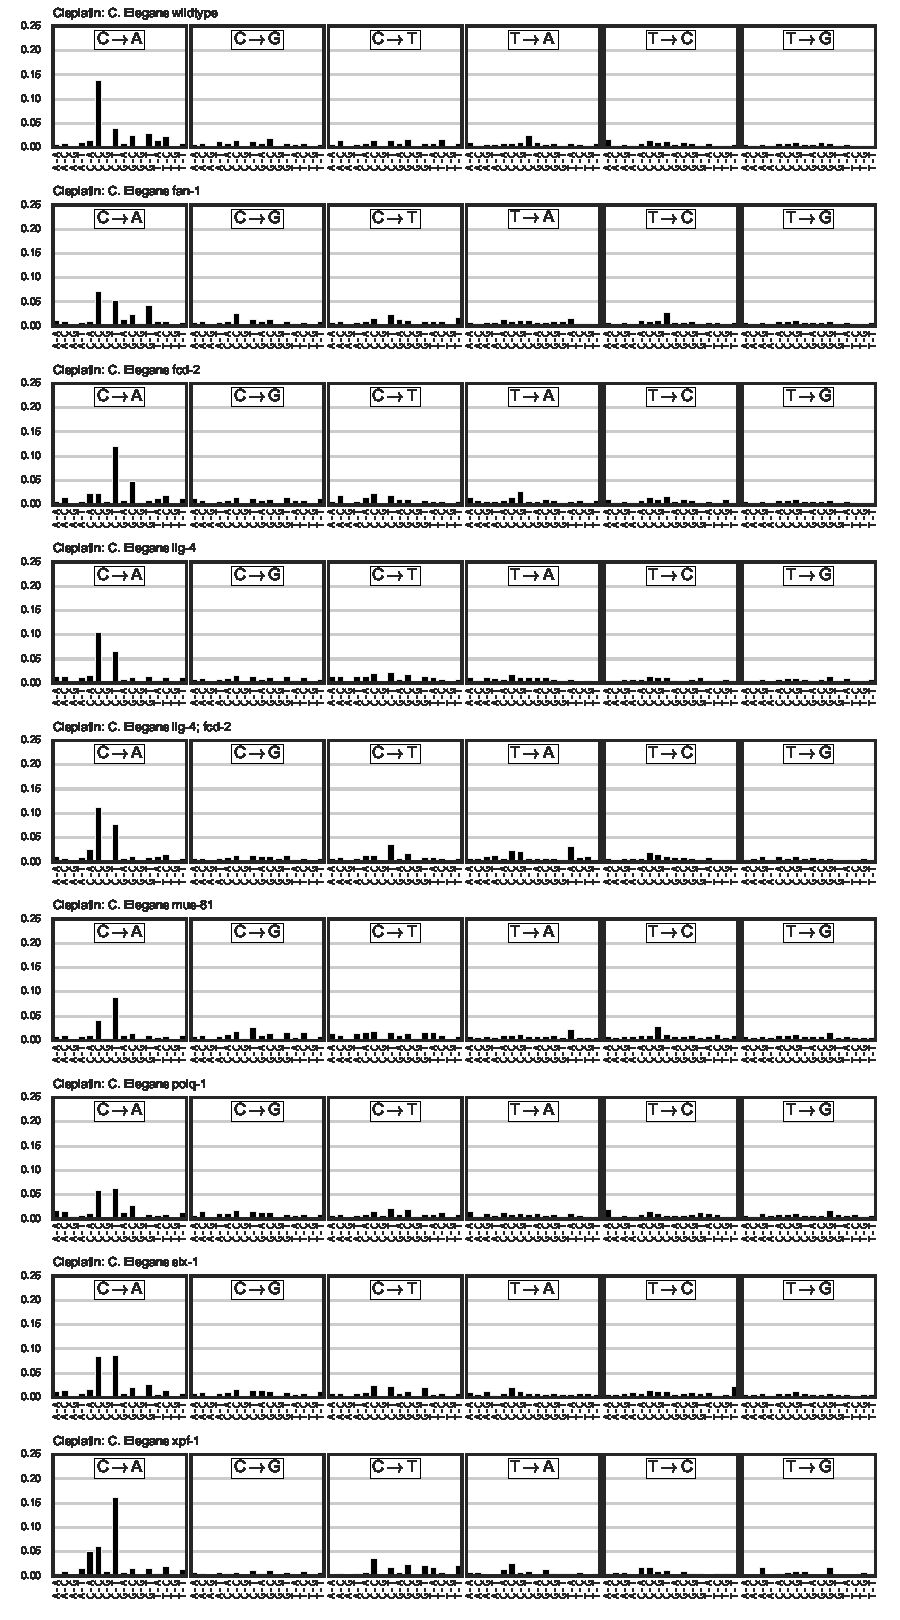
\includegraphics[scale=1.0]{figures/extracted_signatures_worm.pdf}
\caption{Mutational signature extracted from Meier et al.~\cite{Meier_2014}}
\label{fig:supp_extracted_signatures_worm}
\end{figure}

\begin{figure}
\centering
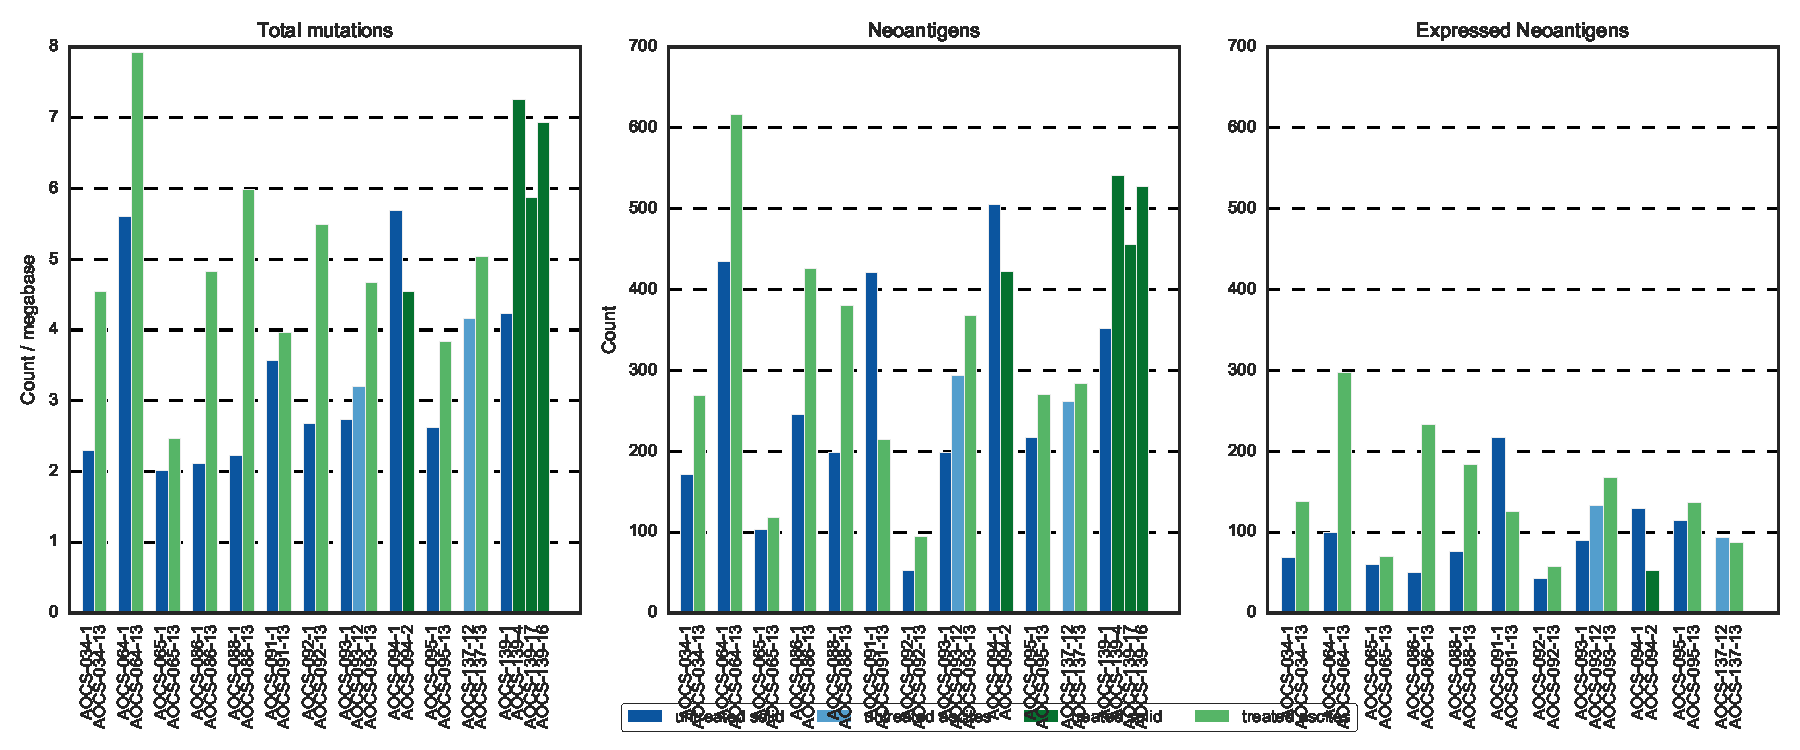
\includegraphics[scale=1.0]{figures/paired_counts.pdf}
\caption{Mutations, neoantigens, and expressed neoantigens for the patients with paired pre- and post-chemotherapy samples. All patients with paired samples received AMCT.}
\label{fig:supp_paired}
\end{figure}

\begin{figure}
\centering
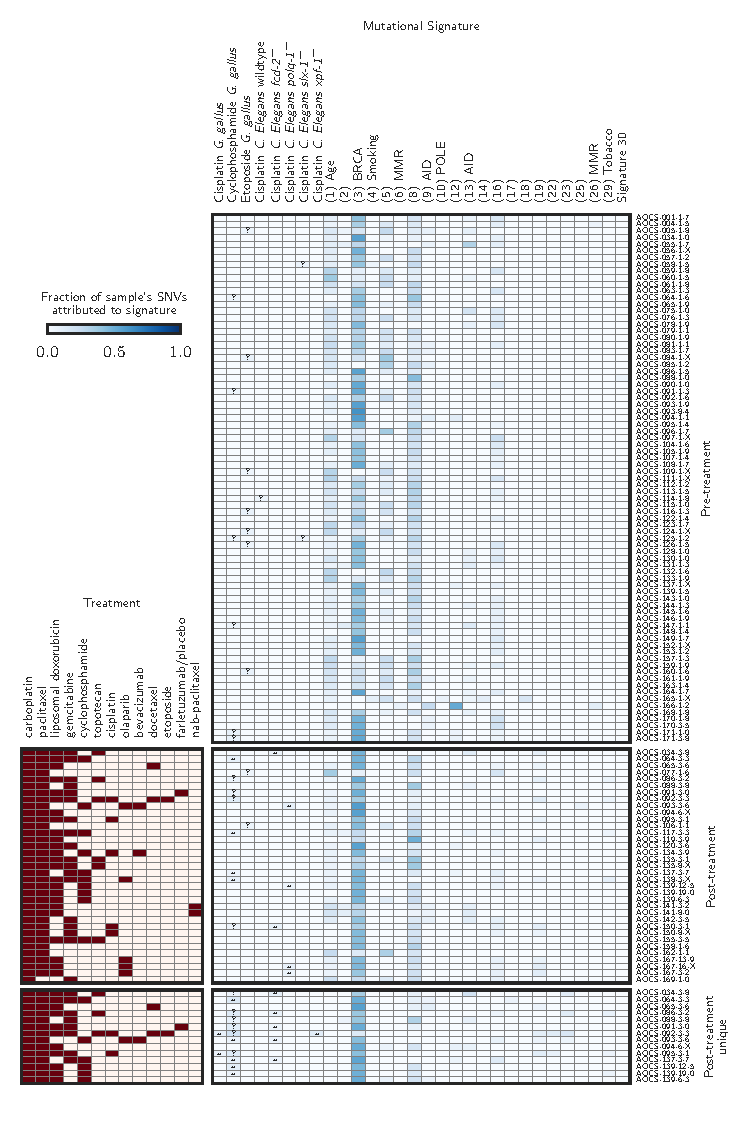
\includegraphics[scale=1.0]{figures/supplementary_signatures.pdf}
\caption{\textbf{Mutational signature deconvolutions for all samples.} The symbols are as in main text Figure~\ref{fig:signatures}.}
\label{fig:supp_signatures}
\end{figure}

\begin{figure}
\centering
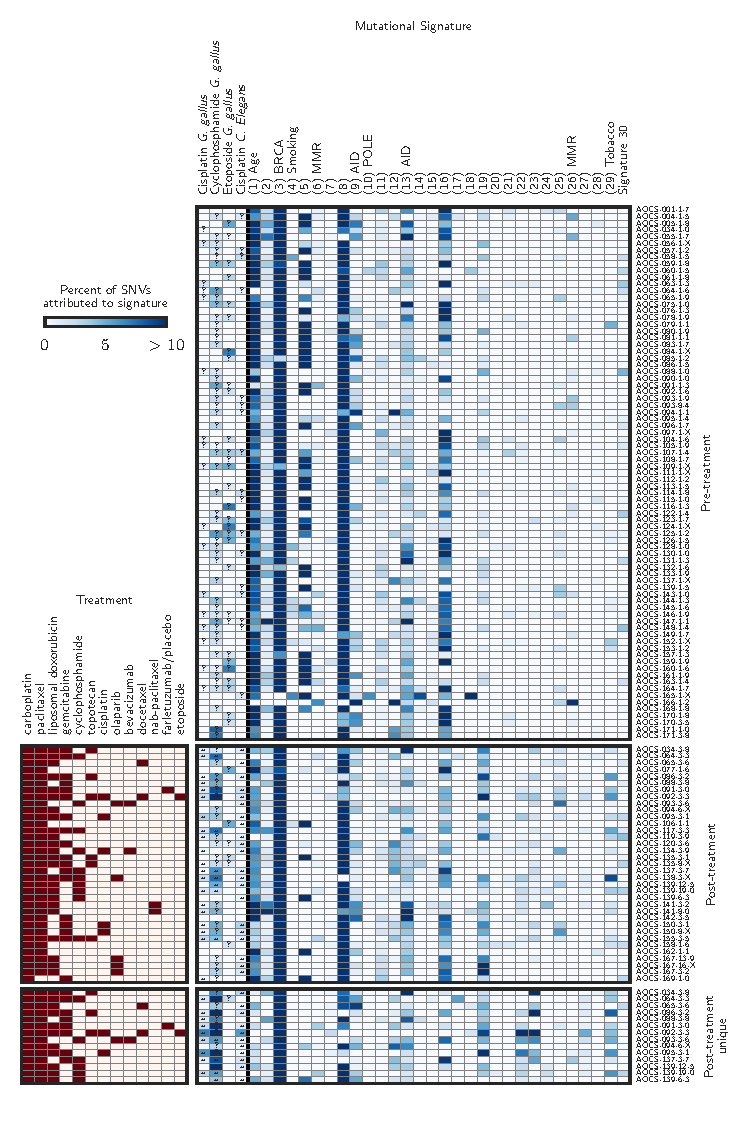
\includegraphics[scale=1.0]{figures/supplementary_signatures_no_cutoff.pdf}
\caption{\textbf{Mutational signature deconvolutions for all samples, without any minimum threshold.} Signatures accounting for less than the 6\% recommended detection threshold are included. The symbols are as in main text Figure~\ref{fig:signatures}.}
\label{fig:supplementary_signatures_no_cutoff.pdf}
\end{figure}

\FloatBarrier
